\documentclass{SCWorks}

\usepackage[english,russian]{babel}
\usepackage{hyperref}
\usepackage{minted}

% Настройка minted согласно правилам курса
\setminted[cpp]{
    frame=lines,
    framesep=2mm,
    baselinestretch=1.2,
    linenos=true,
    fontsize=\footnotesize,
    tabsize=4
}

\begin{document}

\section*{Введение}
В данной работе рассматривается алгоритм поиска в ширину (Breadth-First Search, BFS) на графах, его математические свойства и программная реализация. Этот подход является основополагающим в теории графов и широко применяется на практике \cite{cormen}.

\section{Математическое описание алгоритма}
Пусть задан граф $G = (V, E)$, где $V$ --- множество вершин, а $E$ --- множество ребер. Для любого неориентированного графа выполняется лемма о рукопожатиях, связывающая степени вершин с количеством ребер:
\begin{equation}
\label{eq:degsum}
\sum_{v \in V} \deg(v) = 2|E|
\end{equation}

Алгоритм BFS позволяет находить кратчайшие расстояния $d(u, v)$ между вершинами в невзвешенном графе. Функция расстояния определяется следующим образом:
\begin{equation}
\label{eq:distance}
d(u, v) = \begin{cases} 
\min \{ |P| : P \text{ --- путь между } u \text{ и } v \}, & \text{если путь существует}, \\
\infty, & \text{в противном случае}.
\end{cases}
\end{equation}

Временная сложность стандартной реализации обхода приведена в формуле \eqref{eq:complexity}:
\begin{equation}
\label{eq:complexity}
T(|V|, |E|) = \mathcal{O}(|V| + |E|)
\end{equation}

\section{Визуализация структуры данных}
Для демонстрации работы алгоритма рассмотрим пример графа. На рисунке \ref{fig:graph} изображена исходная схема связей, а на рисунке \ref{fig:bfs_tree} --- получившееся дерево обхода после выполнения BFS \cite{bfs_origin}.

\begin{figure}[H]
\centering
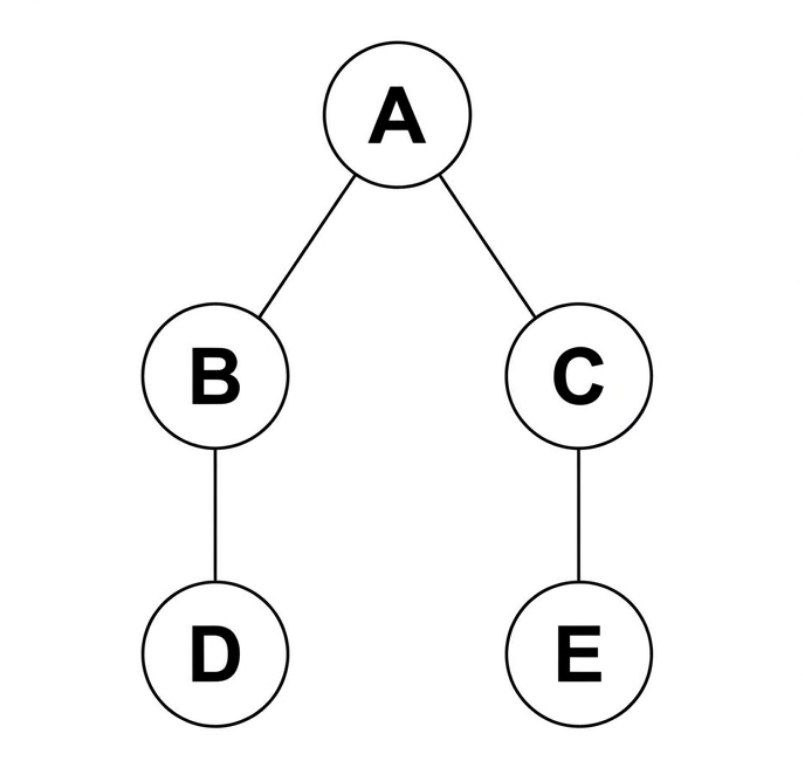
\includegraphics[width=0.4\textwidth]{graph.png}
\caption{Исходный исследуемый граф}
\label{fig:graph}
\end{figure}

\begin{figure}[H]
\centering
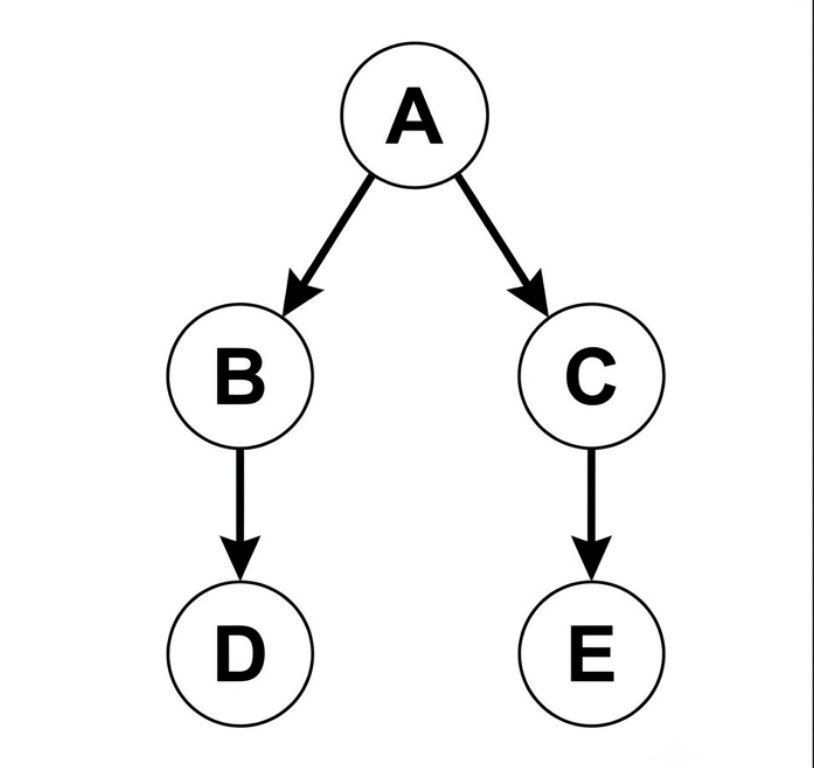
\includegraphics[width=0.4\textwidth]{bfs_tree.png}
\caption{Дерево кратчайших путей (BFS-дерево)}
\label{fig:bfs_tree}
\end{figure}

\section{Анализ сложности}
Поиск в ширину сравнивается с другими алгоритмами поиска путей в таблице \ref{tab:complexity_comp}.

\begin{table}[H]
\centering
\caption{Сравнение алгоритмов поиска кратчайших путей}
\label{tab:complexity_comp}
\begin{tabular}{|l|c|c|c|}
\hline
\textbf{Алгоритм} & \textbf{Временная сложность} & \textbf{Пространственная сложность} & \textbf{Тип графа} \\ \hline
BFS & $\mathcal{O}(|V| + |E|)$ & $\mathcal{O}(|V|)$ & Невзвешенный \\ \hline
Дейкстра & $\mathcal{O}(|V|^2 + |E|)$ & $\mathcal{O}(|V|)$ & Положительные веса \\ \hline
Беллман-Форд & $\mathcal{O}(|V| \cdot |E|)$ & $\mathcal{O}(|V|)$ & Любые веса \\ \hline
\end{tabular}
\end{table}

\section{Программная реализация алгоритма}
Для управления данными используются векторы \texttt{dist} и \texttt{visited}. Очередь \texttt{q}, объявленная как \texttt{std::queue<int>}, управляет порядком обработки вершин. 

Полный исходный код функции представлен в листинге \ref{code:bfs_impl}. Переменная \mintinline{cpp}{current_node} фиксирует текущую извлекаемую вершину.

\begin{listing}[H]
\caption{Реализация алгоритма BFS на языке C++}
\label{code:bfs_impl}
\inputminted{cpp}{bfs.cpp}
\end{listing}

\bibliographystyle{plain}
\bibliography{biblio}

\end{document}
